%!TEX root=./report.tex
\section{EVALUATION}

As a reminder, we have currently seeded the Proctor framework with the task of identifying the correct object model from a database, given a scan of a model in an uncluttered scene.
The detector should output one answer to this problem, although we also evaluate the process by which it arrives at the final answer.
In our evaluations, we care about both accuracy and speed of the detector.

\subsection{Accuracy Dashboard}

We evaluate the correctness of our results via the following scalar values
\begin{itemize}
  \item Percentage of final results that are correct. This gives a rough idea of how well the detector is performing.
  \item The Average Precision (AP), which is the area under the Precision-Recall curve for the registration accuracy of the final result. The AP is one of the most common scalar metrics of performance in computer vision~\cite{pascal-voc-2010}.
  \item Average Rank (AR) of correct model (using preliminary voting results). This number speaks to how well the features can get the right answer without any registration steps.
  \item Area Under the Cumulative Result-within-top-K histogram (AUCR) (using preliminary voting results). This gives a complementary picture to the average rank, as it describes the shape of the histogram instead of merely its mean. The maximum value is $1$, and the minimum value is $0.5$.
\end{itemize}

\begin{figure*}[thpb]
\centering
  \subfloat[Table of scalar measures of performance. The best number in each row is emphasized.]{
\label{tab:PSB_results}
\begin{tabular}{ | l || c | c | c | c | }
\hline
Metric & PFH & FPFH & SHOT & Spin \\
\hline
 \% Correct & 86.25 & \bf 87.50 & 73.75 & 49.35 \\
AP & 0.85 & \bf 0.86 & 0.64 & 0.31 \\
Avg. Rank & 2.23 & \bf 2.16 & 2.23 & 3.45 \\
AUCR & 0.85 & \bf 0.85 & 0.85 & 0.65 \\
\hline
\end{tabular}
  } \\
  \subfloat[Precision-Recall curves, generated by sorting trials by the final registration distances between scene and candidate models.]{
\label{fig:PSB_pr}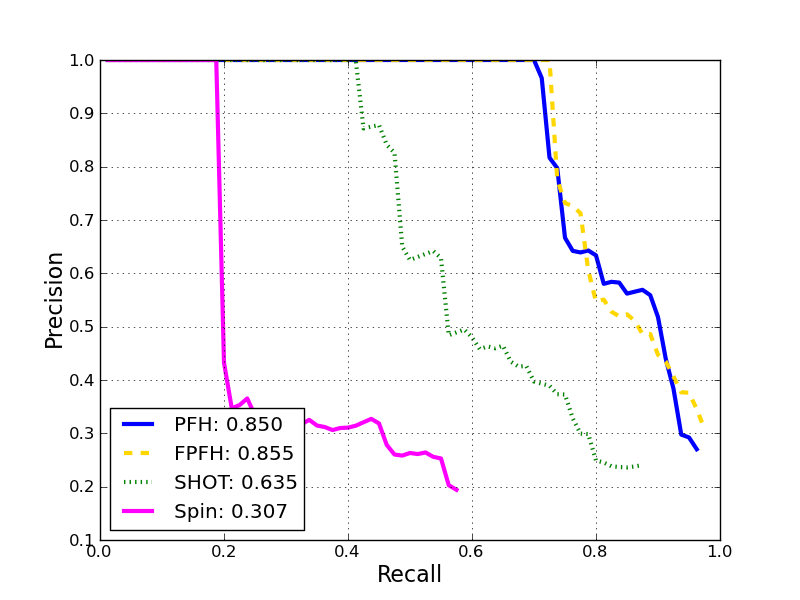
\includegraphics[width=0.45\linewidth]{../figures/PSB/PFH-FPFH-SHOT-SPIN_IMAGE_pr.png}
} \hfill \subfloat[Cumulative rank histogram shows the proportion of trials in which the correct result was fetched by the features in the initial stage.]{
\label{fig:PSB_rankhist}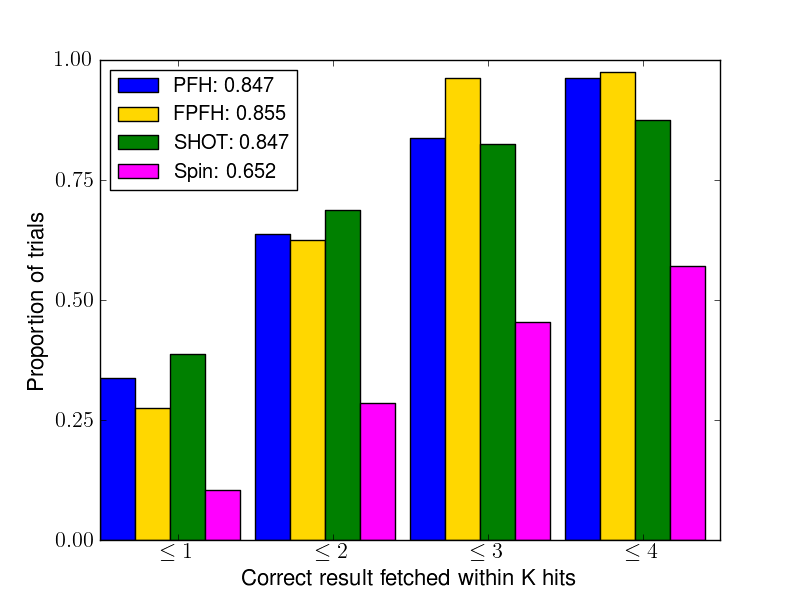
\includegraphics[width=0.45\linewidth]{../figures/PSB/PFH-FPFH-SHOT-SPIN_IMAGE_rankhist.png}
} \\
  \subfloat[PFH]{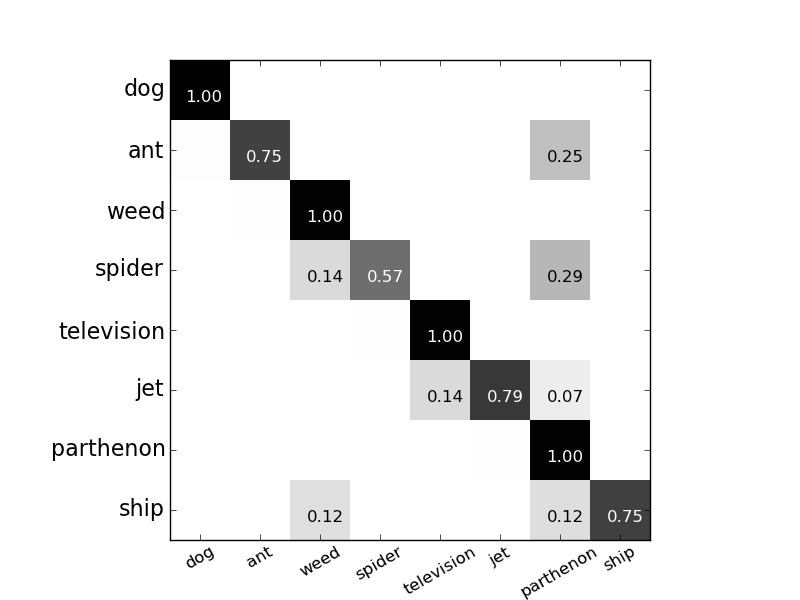
\includegraphics[width=0.45\linewidth]{../figures/PSB/PFH_confmat.png}} \hfill
  \subfloat[FPFH]{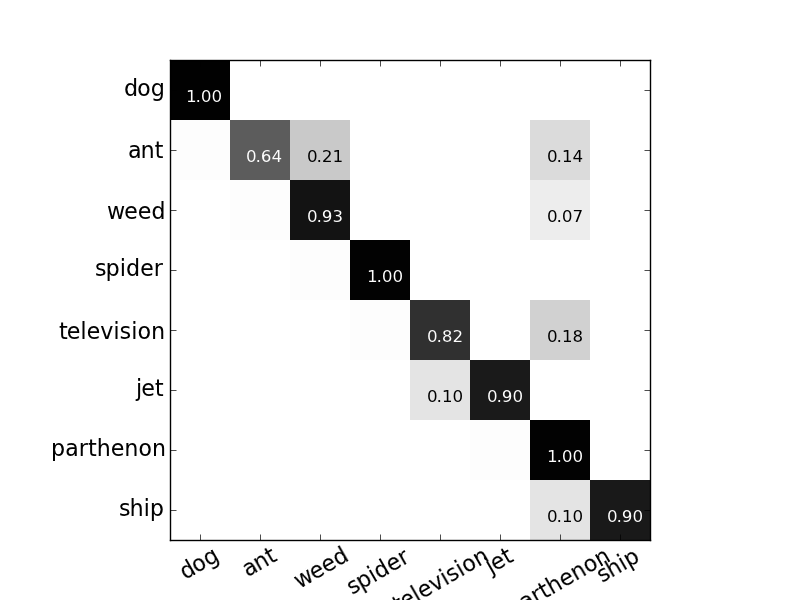
\includegraphics[width=0.45\linewidth]{../figures/PSB/FPFH_confmat.png}}\\
  \subfloat[SHOT]{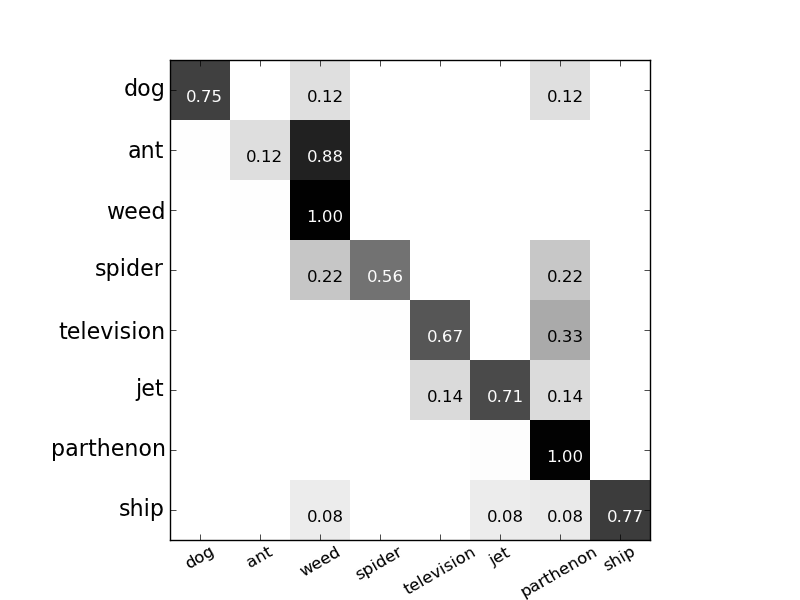
\includegraphics[width=0.45\linewidth]{../figures/PSB/SHOT_confmat.png}} \hfill
  \subfloat[Spin Image]{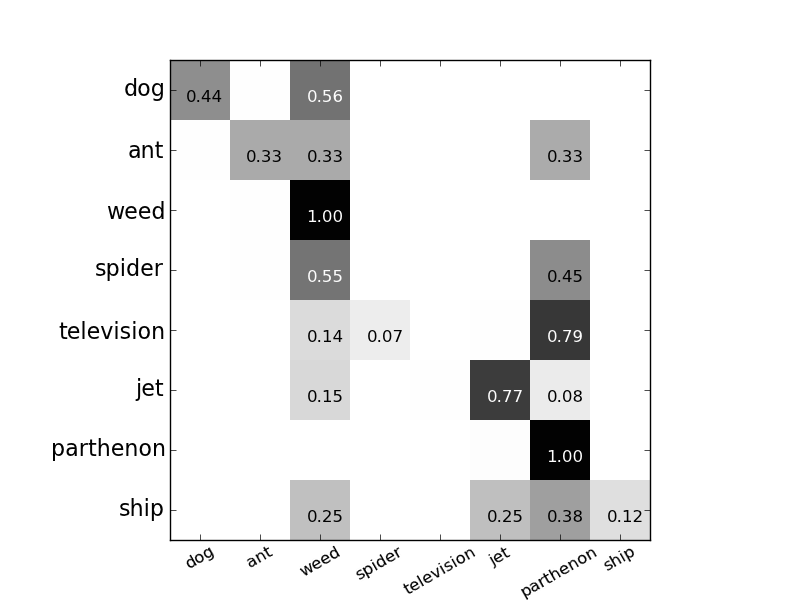
\includegraphics[width=0.45\linewidth]{../figures/PSB/SPIN_IMAGE_confmat.png}}
  \caption{Dashboard for the accuracy-related performance of the different features on the Princeton Shape Benchmark dataset.}
  \label{fig:PSB_dashboard}
\end{figure*}

\begin{figure*}[thpb]
\centering
  \subfloat[Table of scalar measures of performance. The best number in each row is emphasized.]{
\label{tab:WGDB_results}
\begin{tabular}{ | l || c | c | c | c | }
\hline
Metric & PFH & FPFH & SHOT & Spin \\
\hline
 \% Correct & 41.25 & \bf 81.25 & 71.25 & 28.21 \\
AP & 0.26 & \bf 0.75 & 0.58 & 0.20 \\
Avg. Rank & 4.26 & 2.58 & 2.56 & \bf 1.86 \\
AUCR & 0.66 & 0.83 & \bf 0.83 & 0.67 \\
\hline
\end{tabular}
  } \\
  \subfloat[Precision-Recall curves, generated by sorting trials by the final registration distance to the ground truth.]{
\label{fig:WGDB_pr}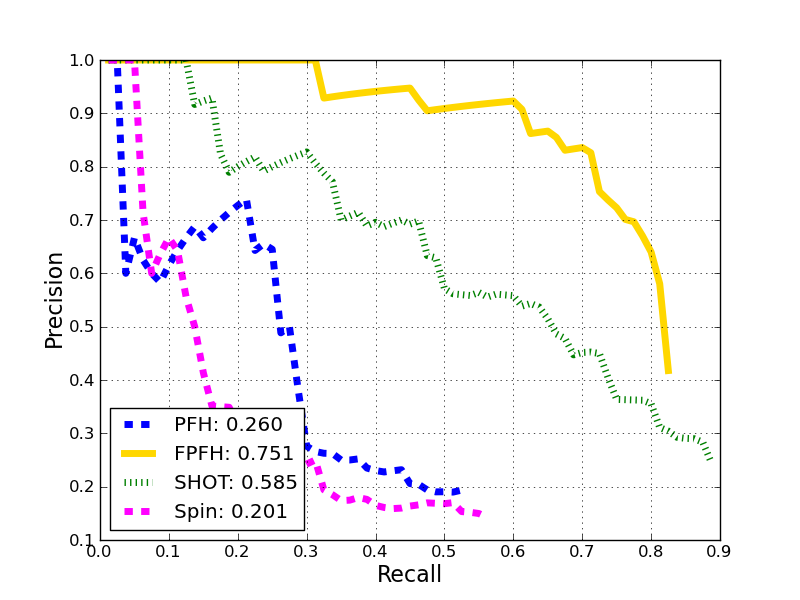
\includegraphics[width=0.45\linewidth]{../figures/WGDB/PFH-FPFH-SHOT-SPIN_IMAGE_pr.png}
} \hfill \subfloat[Cumulative rank histogram shows the proportion of trials in which the correct result was fetched by the features in the initial stage.]{
\label{fig:WGDB_rankhist}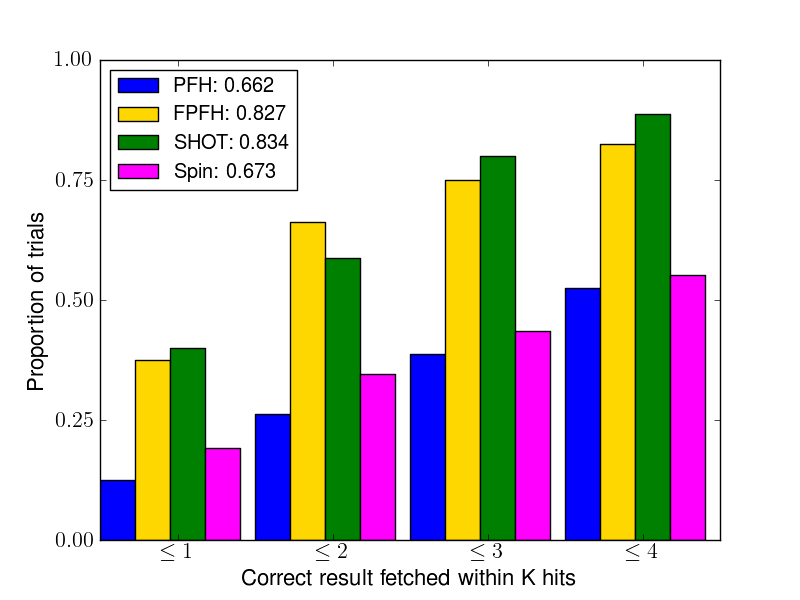
\includegraphics[width=0.45\linewidth]{../figures/WGDB/PFH-FPFH-SHOT-SPIN_IMAGE_rankhist.png}
} \\
  \subfloat[PFH]{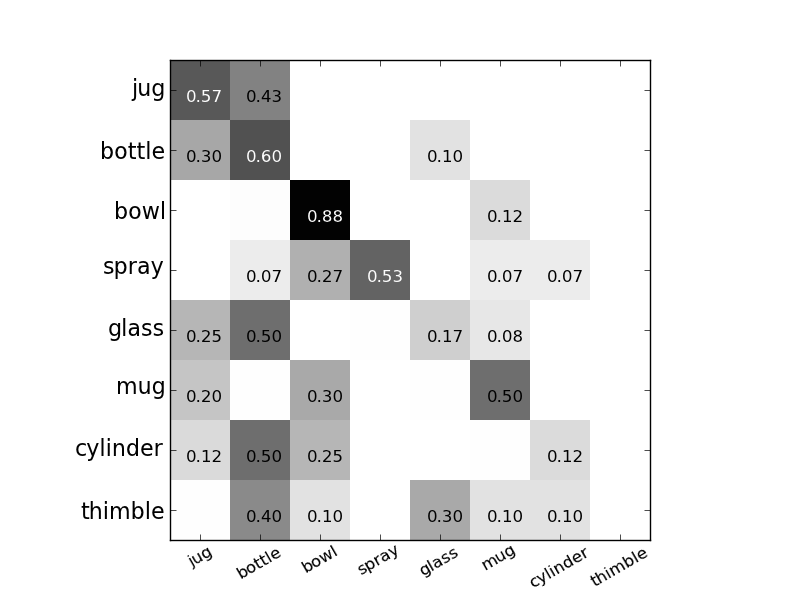
\includegraphics[width=0.45\linewidth]{../figures/WGDB/PFH_confmat.png}} \hfill 
  \subfloat[FPFH]{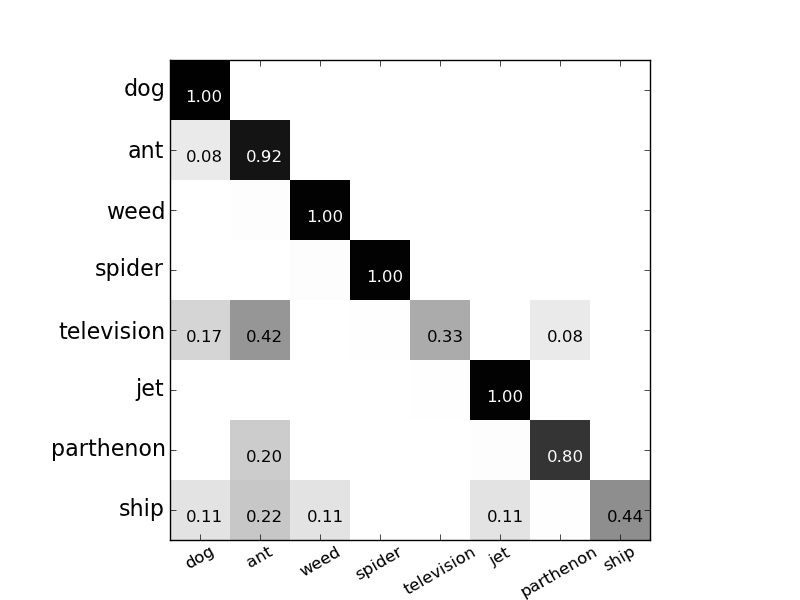
\includegraphics[width=0.45\linewidth]{../figures/WGDB/FPFH_confmat.png}}\\
  \subfloat[SHOT]{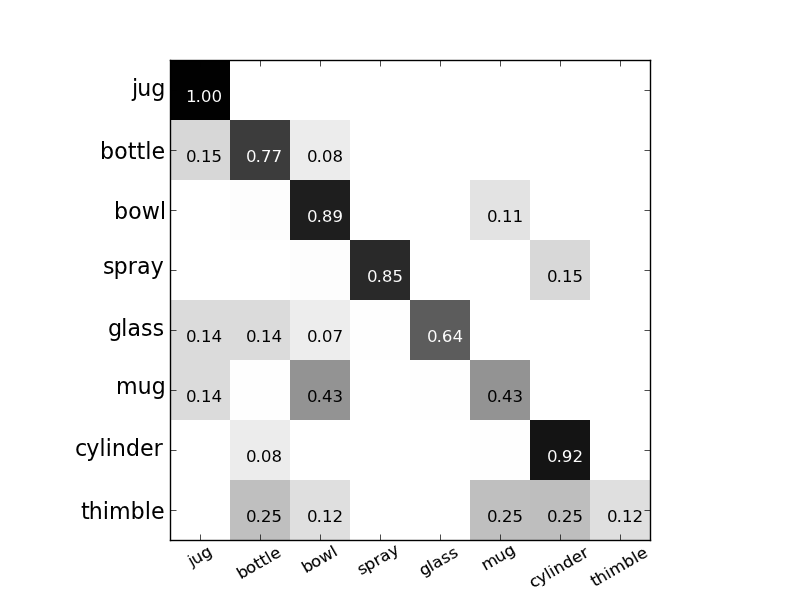
\includegraphics[width=0.45\linewidth]{../figures/WGDB/SHOT_confmat.png}} \hfill
  \subfloat[Spin Image]{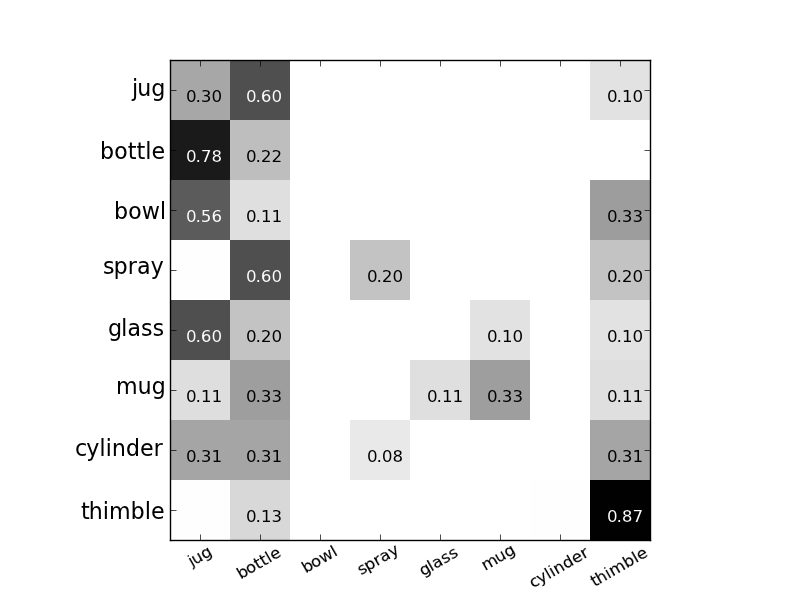
\includegraphics[width=0.45\linewidth]{../figures/WGDB/SPIN_IMAGE_confmat.png}}
  \caption{Dashboard for the accuracy-related performance of the different features on the Willow Garage Grasping dataset.}
  \label{fig:WGDB_dashboard}
\end{figure*}

These scalar metrics, in table form, form one part of our Accuracy Dashboard, seen in~\autoref{fig:PSB_dashboard} for the Princeton Shape Benchmark.
The idea of the Dashboard is that each run of Proctor generates this complete set of results, all available in one place.
Proctor outputs all figures and data for the dashboard, and generates an HTML page and a PDF document tying them together.
In fact, Figures \ref{fig:PSB_dashboard} and \ref{fig:WGDB_dashboard} are examples of such
automatically generated documents---we simply inserted it into this
paper's source.

In addition to the scalar metrics, which are useful for a summary comparison of different features or algorithms, the Dashboard provides visualization of three things:
\begin{itemize}
  \item For each feature, the confusion matrix between final results. This can be a useful tool to understand the behavior of the detector and a source of information for tuning the approach.
  \item Precision-Recall curves comparing all features. It is valuable to know whether a feature results in High-Precision, Low-Recall performance (such as requested by the Solutions in Perception Challenge \cite{SIPC2011}) or Low-Precision, High-Recall performance. By itself, the AP does not provide this information.
  \item The cumulative result-within-top-K histogram comparing all features. Once again, although we have both the Average Rank and the AUCR measures, it is valuable to see the shape of the histogram.
\end{itemize}

\subsection{Timing Dashboard}

Correctness is but one side of performance.
Timing information is crucial when selecting which feature to use for a task: a real-time robotics application has fundamentally different constraints than an offline large database matching application.

The Timing Dashboard, seen in~\autoref{fig:PSB_timing} for the Princeton Shape Benchmark, provides both overall and detailed information about where time is spent in the pipeline.
This data can allow focused work on fast feature extraction and on algorithms to speed up matching, such as locality-sensitive hashing \cite{Frome2004}.

The top-level view of timing is provided by part (a) of the Timing Dashboard, which compares the total time spent in training and testing for the evaluated features.

For training, this can further be broken down into finding the keypoints at which to do feature description, doing the feature description, and constructing the KD-Tree of features.
As it happens, only the feature description step has any significant time investment.
As our reported implementation constructs a dense grid of keypoints at which each feature descriptor is estimated, there is virtually no time spent on finding keypoints.
For different types of keypoints, this may of course change. %and our plotting system is robust to it.
The KD-Tree construction is extremely fast, as we are making use of FLANN~\cite{FLANN}.

Testing can be broken down into finding the keypoints, feature description, collecting votes from features, finding initial alignments from the features, and finally doing Iterative Closest Point \cite{BeslMcKay} on the best few alignments (those that are past a distance threshold).
Since these steps all incur meaningful time costs, we present the breakdowns visually in part (b) of the Dashboard (see~\autoref{fig:PSB_timing} for the Princeton Shape Benchmark).

In this paper, in all cases, the tests were run on a 2.50 GHz Intel Core2 Quad Q9300 with 4 GB of RAM.

\begin{figure*}[thpb]
\centering
\subfloat[Total time spent in training and testing phases of the pipeline.]{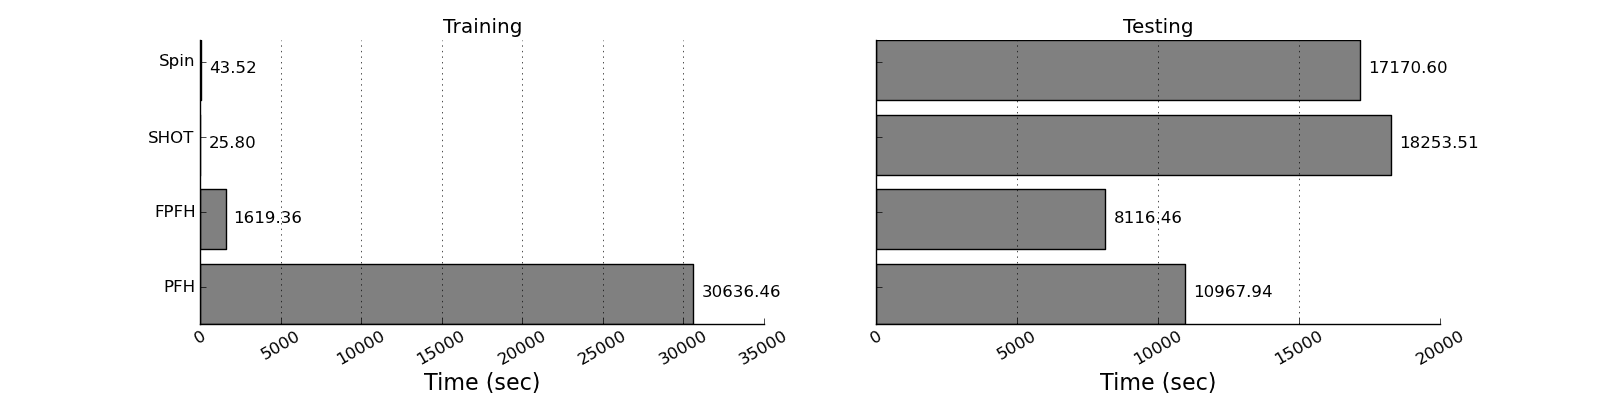
\includegraphics[width=0.95\linewidth]{../figures/PSB/PFH-FPFH-SHOT-SPIN_IMAGE_timing_overview.png}} \\
\vspace{1em}
\subfloat[Breakdown of where time is spent in the testing phase.]{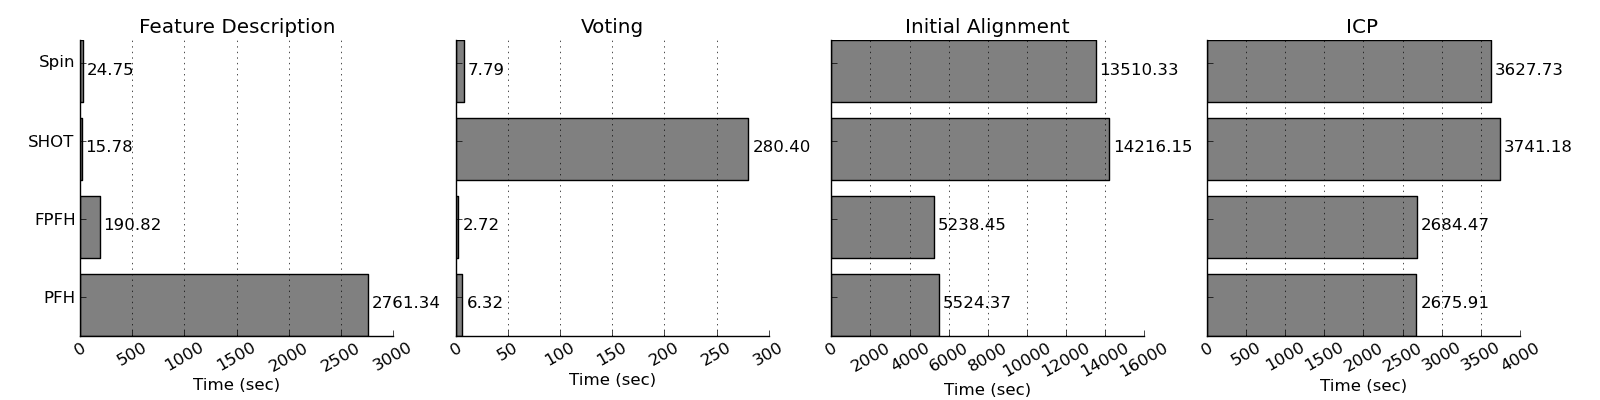
\includegraphics[width=0.95\linewidth]{../figures/PSB/PFH-FPFH-SHOT-SPIN_IMAGE_timing_test_panel.png}} 
\caption{Timing results on the Princeton Shape Benchmark dataset.}
\label{fig:PSB_timing}
\end{figure*}

\begin{figure*}[thpb]
\centering
\subfloat[[Total time spent in training and testing phases of the pipeline.]{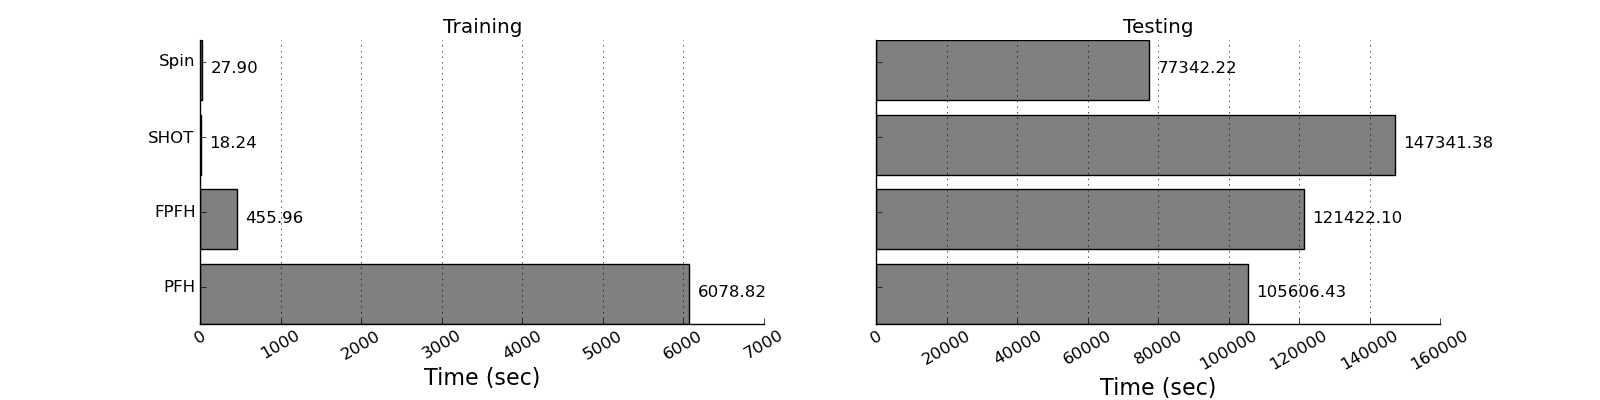
\includegraphics[width=0.95\linewidth]{../figures/WGDB/PFH-FPFH-SHOT-SPIN_IMAGE_timing_overview.png}}
\vspace{1em}
\subfloat[Breakdown of where time is spent in the testing phase.]{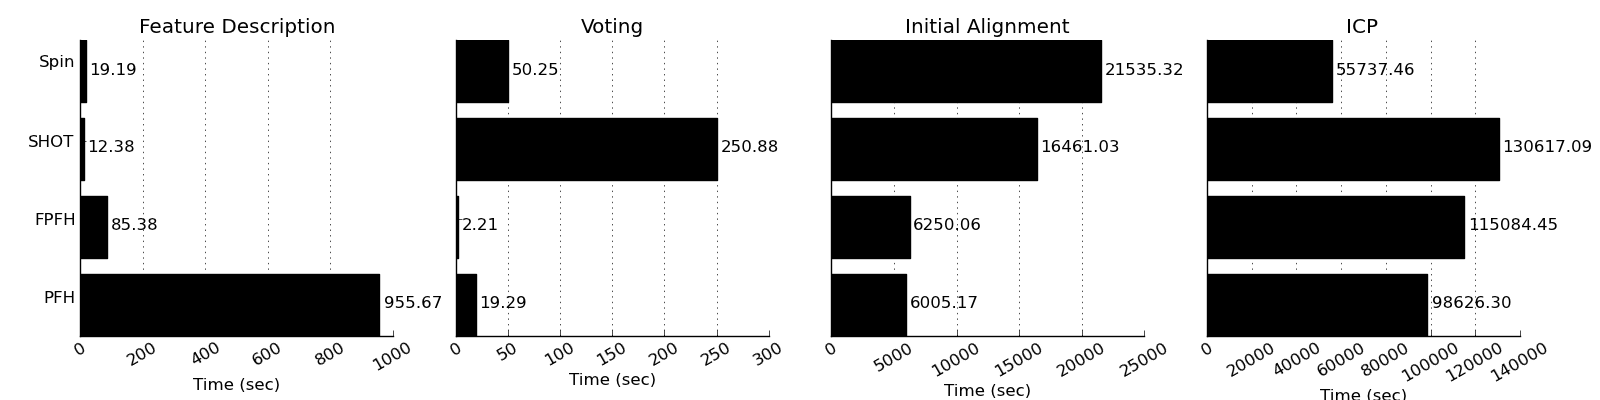
\includegraphics[width=0.95\linewidth]{../figures/WGDB/PFH-FPFH-SHOT-SPIN_IMAGE_timing_test_panel.png}} 
\caption{Timing results on the Willow Garage Grasping dataset.}
\label{fig:WGDB_timing}
\end{figure*}

\subsection{Results}
The results on two datasets, the Princeton Shape Benchmark (PSB), and the Willow Garage Grasping (WGG) Dataset, are presented in Figures \ref{fig:PSB_dashboard}, \ref{fig:PSB_timing}, \ref{fig:WGDB_dashboard}, and \ref{fig:WGDB_timing}.

We can see that across the board, FPFH is an excellent feature.
It performs best in the \% Correct and AP metrics for both datasets, although SHOT does better with the voting classifier in evaluations for the WGG dataset.
From the timing breakdown plots, we can note that although the description is fast for SHOT, the voting stage is the slowest among all the features due to its large signature size.

Although its voting performance is best, SHOT's performance drops after the registration step.
This is a valuable problem identification, as we are now aware of the feature's speed and accuracy in voting, and only need to work on the initial alignment and registration steps if we want to boost its performance.

Proctor enables this kind of problem identification, and the Dashboards allow constant monitoring of progress as solutions are tried.
